% Hola Nati, te quedó LiveShare abierto. Perdí

\documentclass[11pt]{article}
\usepackage[a4paper, margin=2.54cm]{geometry}
\usepackage[utf8]{inputenc}
\usepackage[spanish, mexico]{babel}
\usepackage[spanish]{layout}
\usepackage{amsmath}
\usepackage{amssymb}
\usepackage{amsfonts}
\usepackage{tikz}
\usepackage{enumerate}
\usetikzlibrary{arrows}

\title{
    Entrega Práctica de Ontología \\
    \large Introducción a la Inteligencia Artificial}
\author{Juan Ignacio Farizano}
\date{}

\begin{document}
\maketitle
\noindent\rule{\textwidth}{1pt}

\begin{enumerate}[I. ]
  \item Dos clases son disjuntas si una instancia no puede pertenecer a ambas
        clases al mismo tiempo. Como ejemplo en el enunciado podemos mencionar
        los materiales, un material no puede ser una columna de opinión y un
        juego a la vez.
  \item Si un diario es Específico de Fútbol, transitivamente ese diario es un
        Diario Deportivo y a su vez, es un Diario.
  \item Defino los elementos de modelado ontológico
      \begin{itemize}
            \item Conceptos:
                  \begin{itemize}
                        \item Diario
                              \begin{itemize}
                                    \item Diario deportivo
                                    \begin{itemize}
                                          \item Específico de Fútbol
                                          \item Específico de Rugby
                                    \end{itemize}
                              \end{itemize}
                        \item Campo
                              \begin{itemize}
                                    \item Inmuebles
                                    \item Política
                                    \item Negocios
                                    \item Economía
                                    \item Deportes
                              \end{itemize}
                        \item Publicación
                              \begin{itemize}
                                    \item Impresa
                                    \item Virtual
                              \end{itemize}
                        \item Material
                              \begin{itemize}
                                    \item Noticia
                                    \item Columna de opinión
                                    \item Pronóstico
                                    \item Juego
                              \end{itemize}
                  \end{itemize}
            \item Relaciones
                  \begin{itemize}
                        \item Cubre de Diario a Campo
                        \item Realiza de Diario a Publicación
                        \item Contiene de Diario a Material
                  \end{itemize}
            \item Restricciones
                  \begin{itemize}
                  \item En Impresa:
                  \begin{itemize}
                        \item Tinta: de tipo String y posibles valores Negra o Color
                        \item Fondo: de tipo String y posibles valores Blanco o Gris
                  \end{itemize}
                  \item En Virtual:
                  \begin{itemize}
                        \item Página propia: de tipo Bool y posibles valores True o False
                  \end{itemize}
                  \item En Específico de Fútbol:
                  \begin{itemize}
                        \item Especializado en clásicos: de tipo Bool y posibles valores True o False
                  \end{itemize}
                  \item En Noticia:
                  \begin{itemize}
                        \item Título: de tipo String
                        \item Copete: de tipo String
                        \item Cuerpo: de tipo String
                  \end{itemize}
                  \end{itemize}
      \end{itemize}
% \newpage
      \begin{figure}[h!]
            \begin{center}
              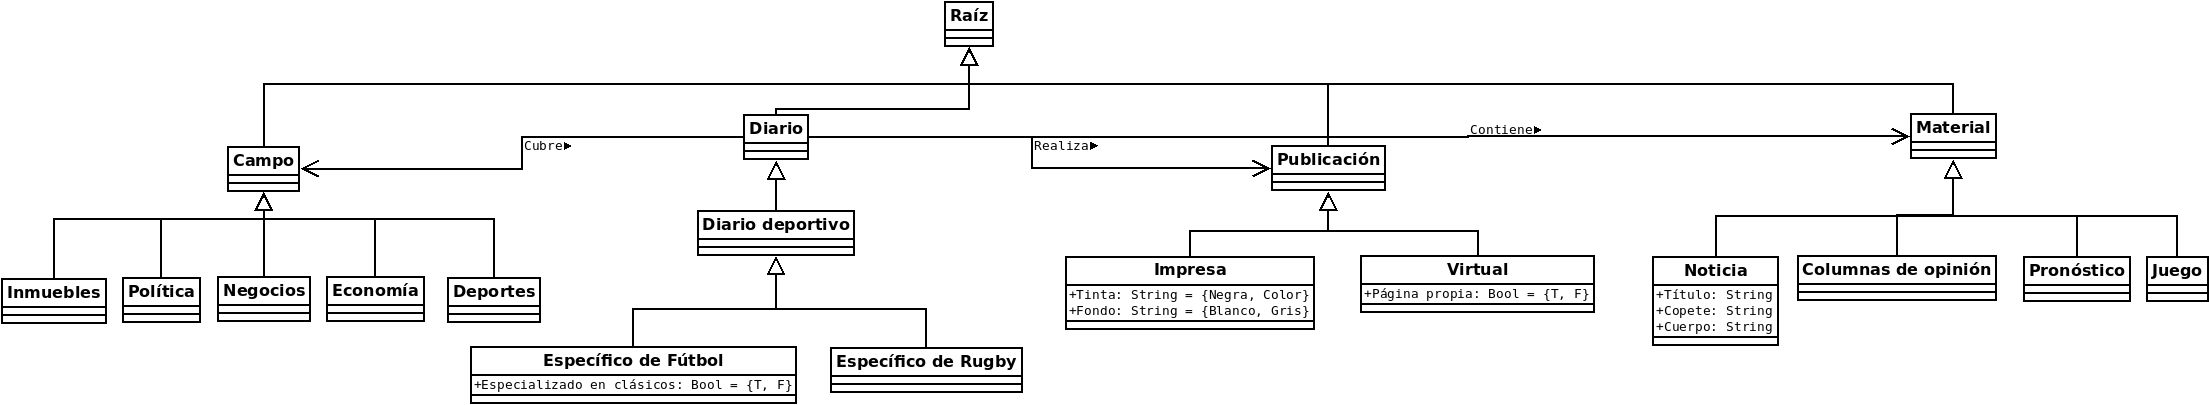
\includegraphics[width=0.99\linewidth]{ontologiaentrega.png}
            \end{center}
          \end{figure}
(Adjunto también la imagen original para poder leer con mayor claridad)
      \item 
            \begin{enumerate}[a.]
                  \item Al ser un diario virtual principalmente enfocado a Política
                  y Economía, podría representarlo como una instancia de la clase
                  Diario, relacionarla mediante la relación Cubre a una instancia
                  "Política Nacional" de la sub-clase Politica de la clase Campo
                  y también relacionarla con una instancia de Economía. 
                  \item Instancia de Noticia relacionada al Diario perfil.com.
            \end{enumerate}

\end{enumerate}


\end{document}